\section{Sprint 2: Comienzo del desarrollo}
\label{sec:comienzo-desarrollo}

Con la propuesta del proyecto ya definida, el desarrollo comenzó con fuerza en febrero de 2026. Poco a poco se fue creando la estructura base de 
la aplicación: modelos, sistema de ingestión de datos, lógica de análisis, y una interfaz mínima para poder hacer
pruebas del flujo completo. La arquitectura hasta este punto era bastante sencilla: una aplicación Django que recibía una URL, descargaba los 
datos de la API, los analizaba y devolvía una propuesta de estructura para el futuro sitio web.

\begin{figure}[H]
    \centering
    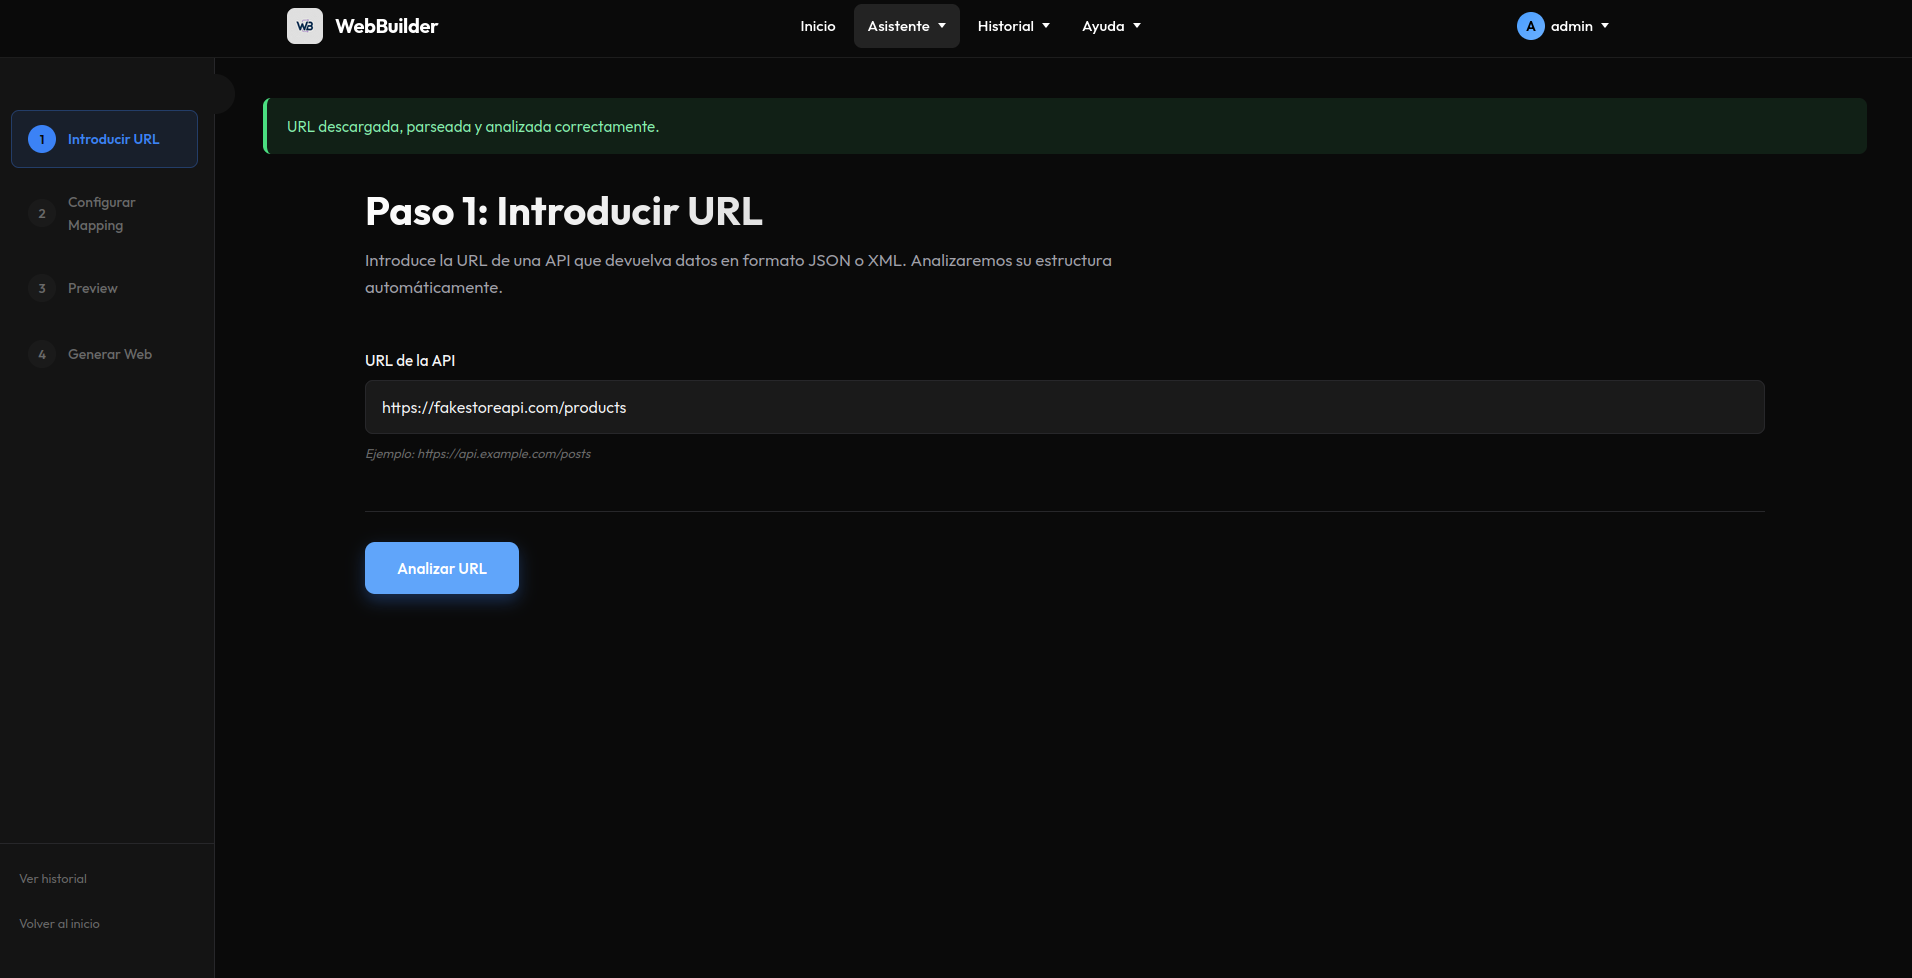
\includegraphics[width=\textwidth]{img/oldversions/urlantigua}
    \caption{Paso 1 del asistente: introducción de la URL de la API}
    \label{fig:urlantigua}
\end{figure}

\begin{figure}[H]
    \centering
    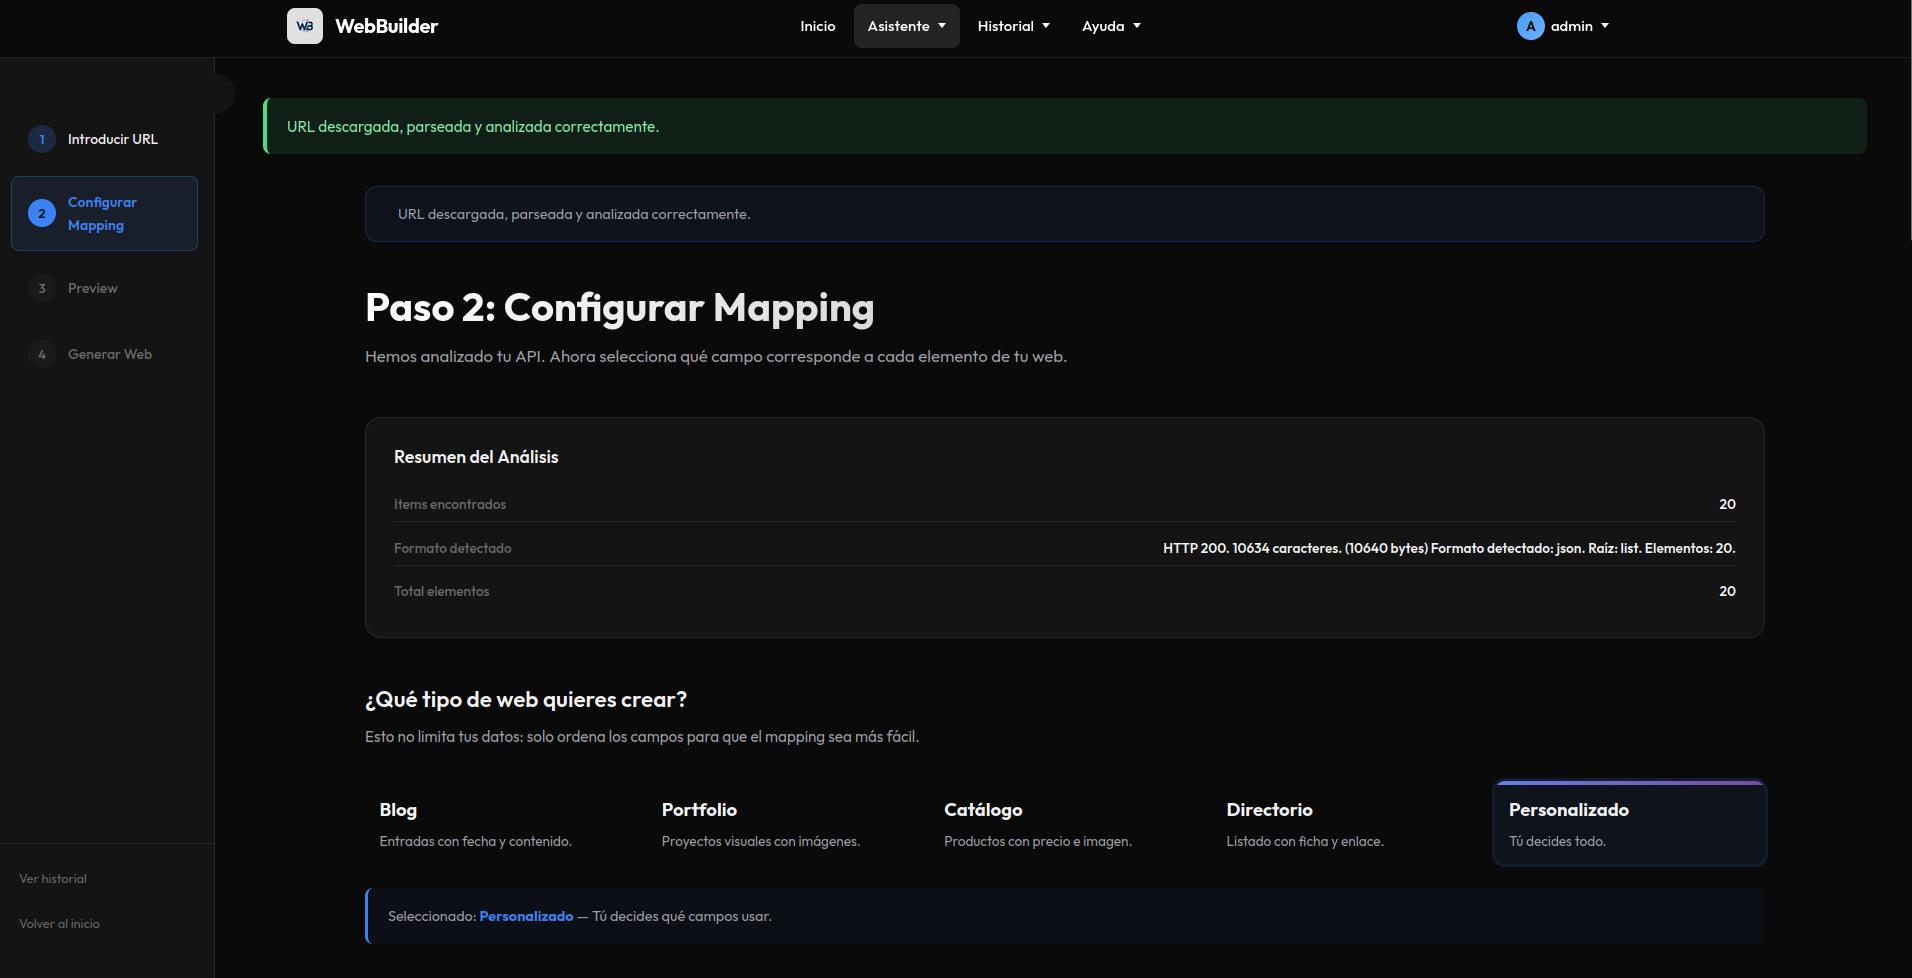
\includegraphics[width=\textwidth]{img/oldversions/heuristicas1}
    \caption{Paso 2 del asistente: configuración del mapping mediante heurísticas}
    \label{fig:heuristicas1}
\end{figure}

\begin{figure}[H]
    \centering
    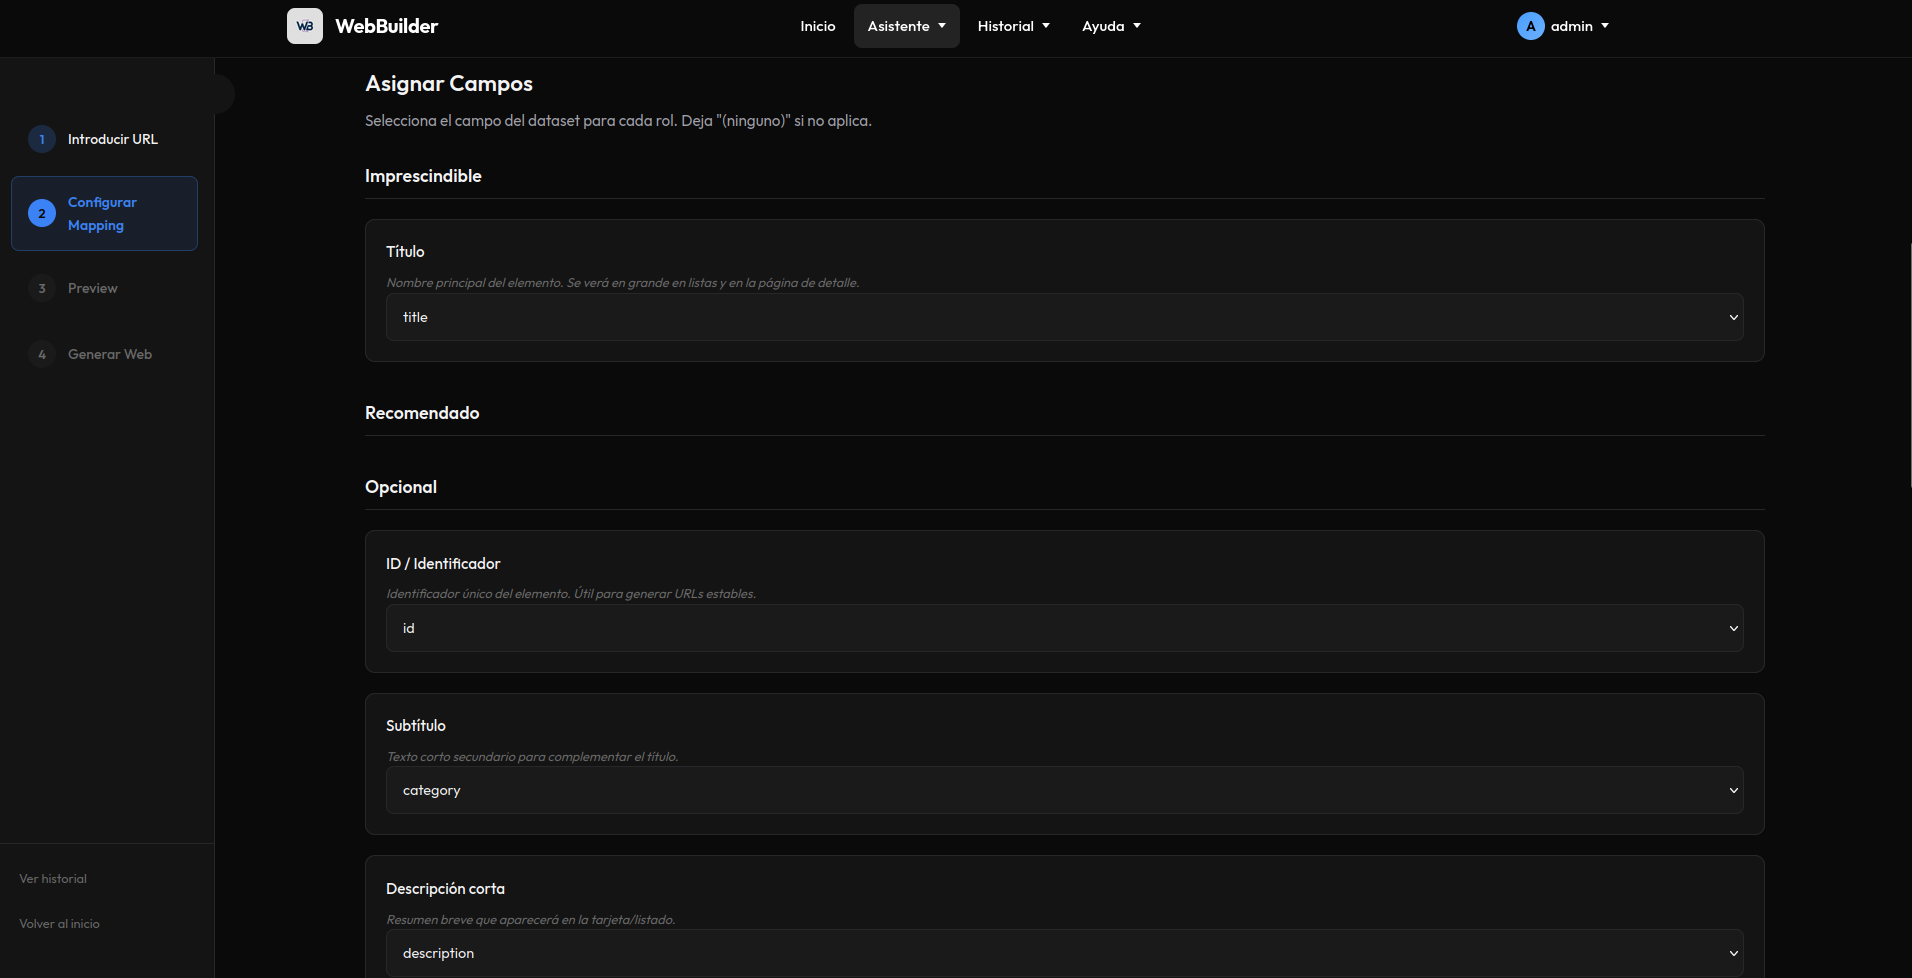
\includegraphics[width=\textwidth]{img/oldversions/heuristicas2}
    \caption{Paso 2 del asistente: asignación manual de campos por roles}
    \label{fig:heuristicas2}
\end{figure}

\subsection{Modelo de datos}
\label{subsec:modelo-datos}

El único modelo de la base de datos en este sprint era \texttt{APIRequest}, que recogía 
los datos de cada petición URL realizada. Sus campos principales se muestran en la 
Tabla~\ref{tab:modelo-apirequest}. Este modelo fue el eje central durante este sprint 
y será la base del análisis durante todo el proyecto.

\begin{table}[H]
    \centering
    \begin{tabular}{|l|l|p{8cm}|}
        \hline
        \textbf{Campo} & \textbf{Tipo} & \textbf{Descripción} \\
        \hline
        url & CharField & URL de la API introducida por el usuario \\
        \hline
        raw\_data & TextField & Datos en crudo descargados de la API \\
        \hline
        parsed\_data & JSONField & Estructura de datos ya parseada \\
        \hline
        status & CharField & Estado del análisis: pending, processed o error \\
        \hline
        field\_mapping & JSONField & Mapping resultante mostrado al usuario \\
        \hline
        created\_at & DateTimeField & Fecha y hora de creación de la petición \\
        \hline
        user & ForeignKey & Usuario propietario del análisis \\
        \hline
    \end{tabular}
    \caption{Campos del modelo APIRequest en la Sprint 2}
    \label{tab:modelo-apirequest}
\end{table}


\subsection{Ingestión de datos}
\label{subsec:ingestion-datos}

El modulo de ingestión de datos, ubicado en \texttt{utils/ingest/} era y será el encargado de validar la URL introducida por el usuario, realizar la descarga del contenido
de forma segura y detectar automáticamente el formato de los datos. La validación comprobaba que la URL procedería de \texttt{http} o \texttt{https}, que fuese
procedente de un dominio válido y que su longitud no superase los 2048 caracteres, límite establecido para evitar ataques mediante URLs maliciosas por su longitud. La descarga se realizaba en modo streaming, es decir, en vez de esperar que
el contenido del archivo se descargue entero, se va leyendo el contenido en fragmentos, cada un con un límite de 1MB, y un timeout de 8 segundos. Conseguimos de 
esta forma evitar que una API con respuestas excesivamente grande nos tumbe o bloquee el sistema.

La detección de formato se realiza inspeccionando los primeros caracteres del contenido de la API, de esta forma se conseguía distinguir entre JSON y XML, que son 
los contenidos manejados hasta este momento, mas adelante en el capítulo~\ref{subsec:nuevos-formatos-entrada} se aumenta el tipo de datos a procesar. En cualquier caso 
siempre se devuelve una estructura Python homogénea, que se utiliza en adelante para el sistema, de forma que no es necesario seguir trabajando con el formato 
original.

\subsection{Detección de la colección principal}
\label{subsection:deteccion-coleccion-principal}

La parte mas compleja de este sprint fue entender la estructura interna de los campos de las distintas APIs. Los campos de las APIs no suelen ser una lista plana de items
en la raíz, es decir, la colección principal no esta expuesta, sino que esta envuelta bajo claves de metadatos como \texttt{results}, \texttt{data} o \texttt{items},
o incluso con varios niveles de profundidad. 

Para resolver esto se implementó un nuevo modulo: \texttt{utils/analysis}, donde se crearon ficheros con funciones importantes como \texttt{find\_main\_items}, la cual recorría recursivamente la estructura de la API, y se evaluaba con un sistema de puntuación propio para sacar la estructura principal.

Cada lista candidata se puntuaba según cinco factores:

\begin{itemize}
    \item \textbf{Densidad de diccionarios}: porcentaje de elementos de la lista que son diccionarios. Las listas con menos de un 55\% de dicts recibían una penalización proporcional, ya que era poco probable que representaran una colección de entidades reales.
    \item \textbf{Tamaño}: listas con más items recibían mayor puntuación, aunque con un límite para evitar que una lista enorme pero trivial se impusiera sobre una colección más pequeña pero más relevante.
    \item \textbf{Consistencia de claves}: si todos los diccionarios de la lista compartían aproximadamente las mismas claves, era muy probable que representaran entidades del mismo tipo. Se calculaba como el promedio de claves propias de cada item sobre la unión de todas las claves observadas.
    \item \textbf{Bonus por claves semánticas}: si los campos de la colección incluían nombres típicos de contenido como \texttt{title}, \texttt{name}, \texttt{id},    \texttt{description} o \texttt{image}, se añadía una bonificación proporcional al número de coincidencias.
    \item \textbf{Penalización por profundidad}: los paths muy anidados o que pasaban por índices numéricos se penalizaban para favorecer colecciones cercanas a la raíz, que solían ser las más relevantes.
\end{itemize}

Al finalizar este scoring, se seleccionaba la lista con mayor puntuación como 
colección principal, junto con la ruta dentro de la estructura original. En la 
Figura~\ref{fig:sistema-scoring} se muestra cómo los cinco factores se combinan 
en la función de scoring para obtener la colección principal.

\begin{figure}[H]
    \centering
    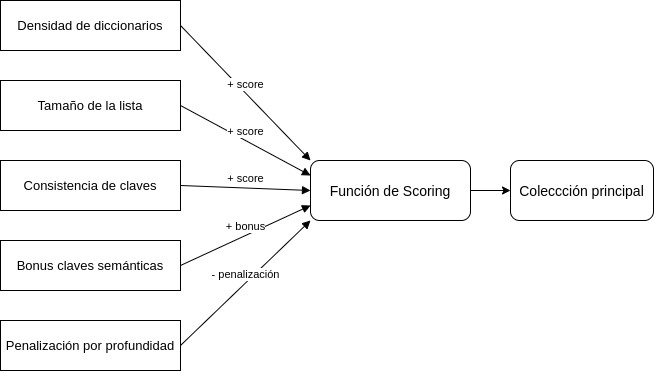
\includegraphics[width=0.7\textwidth]{img/disenoimplementacion/sistemascoring}
    \caption{Sistema de scoring para la detección de la colección principal}
    \label{fig:sistema-scoring}
\end{figure}


\subsection{Sugerencia automática}
\label{subsec:sugerencia-automatica}

Una vez localizada la colección principal, se realizo la implementación del nuevo fichero \textbf{utils/mapping.py}, encargado de sugerir automáticamente que campos
del dataset debían ocupar cada rol: fecha, id, descripción, etc. Para ello se utilizaba un catalogo predefinido que asociaba cada rol con sus nombres más habituales.
Por ejemplo un campo llamado \texttt{published\_at}, obtenía un alto score para el rol fecha ya que contenía la subcadena \texttt{published}.
Además de la comparación por nombre, el sistema añadía score extra si el tipo del campo observado coincidía con el tipo esperado en el rol.

Para evitar que la misma clave del dataset se asignara como primera sugerencia de varios roles a la vez, se implementó una función llamada \texttt{suggest\_mapping}, que aplicaba una asignación por orden de prioridad: primero se reservaba la mejor clave para el rol \texttt{id}, luego para \texttt{title}, luego para \texttt{description}, y así sucesivamente. Esto reducía la repetición de sugerencias y hacía el mapping resultante más útil para el usuario, sin embargo, ocurrían errores como que algunos campos se quedasen vacíos o que al asignarse por orden de prioridad, algunos campos sueltos se asignasen a roles
que no tenían relación.



\subsection{Elección pagina}
\label{subsec:eleccion-pagina}

Para guiar mejor al usuario durante el proceso de mapping, se añadió un sistema de perfiles de intención en \texttt{intents.py}. El usuario podía indicar si quería construir un blog, un portfolio, un catálogo o un directorio, y el sistema reordenaba los roles y ajustaba cuáles eran obligatorios, recomendados u opcionales según ese tipo de sitio.
Se puede observar en las Figuras~\ref{fig:heuristicas1} y~\ref{fig:heuristicas2} 
cómo el sistema solicitaba al usuario configurar el tipo de pagina y los campos.

\subsection{Calidad del mapping}
\label{subsec:calidad-mapping}
Además, se implementó un sistema de puntuación de calidad del mapping en \texttt{mapping.py}, que evaluaba de 0 a 100 el mapping introducido por el usuario teniendo en cuenta si había asignado los roles más importantes, si existían duplicados entre roles críticos y qué campos quedaban vacíos. El resultado se mostraba al usuario con una etiqueta cualitativa: \emph{Excelente}, \emph{Bueno}, \emph{Aceptable} o \emph{Mejorable}.


\subsection{Tests}
\label{subsec:test1}

Desde el primer sprint se escribieron tests para los cuatro módulos principales 
del sistema heurístico, organizados en ficheros independientes: 
\texttt{test\_analysis}, \texttt{test\_mapping}, \texttt{test\_normalizer} 
y \texttt{test\_parsers}. Estos test cubrían casos como la detección de colecciones anidadas, la asignación de roles por prioridad, la normalización de valores y el parseo seguro de XML. Esto permitió verificar el comportamiento del sistema de scoring con datasets variados, detectando casos en los que las heurísticas fallaban antes de que llegaran al usuario.

\subsection*{Limitaciones del enfoque heurístico} 
\label{subsec:limitaciones1}

Conforme se probaba el sistema con datasets reales muy distintos entre sí, los límites del enfoque heurístico se fueron haciendo evidentes. Una API de plantas medicinales, una de personajes de ficción y una de productos de e-commerce tienen nomenclaturas de campos completamente diferentes, y un sistema de reglas fijas no podía cubrir todos los casos con la misma fiabilidad. Cuando los nombres de los campos no coincidían con los campos de la API, el mapping era genérico y malo para el usuario. El sistema funcionaba razonablemente bien con APIs convencionales y con campos estándar, pero fallaba ante cualquier dataset con nombres o estructura poco habituales. Esta limitación fue la que motivó el cambio de enfoque descrito en el siguiente sprint.


